\chapter{Current-State Analysis}

\section{Architecture Overview}

nopCommerce follows an onion architecture, where all dependencies point inward toward the
core. The solution is split into four main layers: \texttt{Nop.Core}, \texttt{Nop.Data},
\texttt{Nop.Services}, and the presentation layer (\texttt{Nop.Web} and
\texttt{Nop.Web.Framework}).

\begin{figure}[h]
\centering
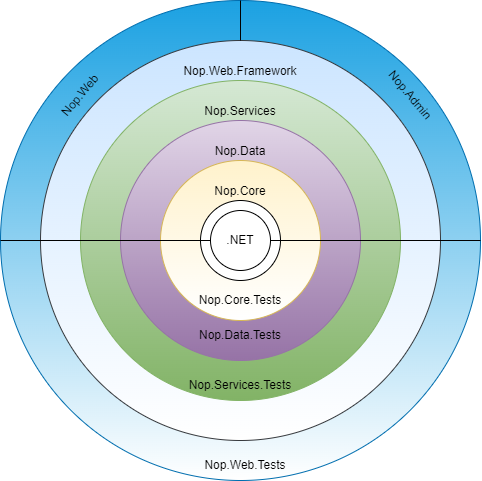
\includegraphics[width=0.68\textwidth]{images/nopCommerceArchitecture.png}
\caption{Current layered/onion architecture of nopCommerce.}
\label{fig:current-nopcommerce-architecture}
\end{figure}

Each layer has a specific role:

\begin{itemize}
\item \textbf{\texttt{Nop.Core}}: The innermost layer. Contains domain entities, caching,
events, and helper classes shared across the whole solution. It has no dependencies on any
other project. Key Scenario C entities live here: \texttt{Order}, \texttt{OrderItem},
\texttt{Product}, \texttt{ProductWarehouseInventory}, \texttt{StockQuantityHistory},
\texttt{Warehouse}, and \texttt{Shipment}.

\item \textbf{\texttt{Nop.Data}}: Separates data-access logic from business objects.
nopCommerce uses a Linq2DB Code-First approach, with FluentMigrator for schema migrations and
Fluent API for persistence mappings.

\item \textbf{\texttt{Nop.Services}}: The outermost layer of the Application Core. It holds
business logic, validations, and calculations, and uses a repository pattern to expose
features to layers above it. This is where order processing, inventory adjustment, shipping,
and checkout logic live. Key services for Scenario C are \texttt{OrderProcessingService},
\texttt{IShipmentService}, \texttt{IProductService}, and \texttt{IStockQuantityHistoryService}.

\item \textbf{\texttt{Nop.Web}} and \textbf{\texttt{Nop.Web.Framework}}: The presentation
layer. \texttt{Nop.Web} contains controllers, models, views, and the storefront and admin
area. \texttt{Nop.Web.Framework} is a shared class library with common presentation logic
used by both the public site and the admin panel. Controllers reference only services, never
repositories directly, which provides a clean seam for adding integration boundaries without
touching the presentation layer.

\item \textbf{Plugins}: Loaded as separate Visual Studio projects and extend nopCommerce for
payments, shipping, authentication, search, and other integrations. They run inside the same
runtime as the monolith and share its process lifecycle.
\end{itemize}

\section{How a Purchase Works Today}

A customer order flows from the storefront controllers in \texttt{Nop.Web} down through
\texttt{Nop.Services}. \texttt{OrderProcessingService} creates the order, adjusts inventory,
persists state via repositories, and publishes internal events like \texttt{OrderPlacedEvent}.
Shipment updates follow later through shipment services, which update order status and trigger
notification events.

This works cleanly when nopCommerce owns the full picture. It breaks down when an external
warehouse, POS, or carrier system owns part of the order's lifecycle and may be slow,
unavailable, or return conflicting data.

The internal event system publishes events in-process to registered consumers and awaits each
one. If a consumer fails, the error is logged and execution continues. There is no message
broker and no standard durable integration retry, replay, or dead-letter mechanism. This is
fine for cache invalidation or plugin reactions, but it is not sufficient for reliable
integration with external systems.

\section{Scenario C Readiness Assessment}

The table below classifies each Scenario C-relevant capability as ready to use, ready but
requiring extension, or missing and needing to be built. This assessment drives the scope of
the target architecture defined in subsequent chapters.

\begingroup
\small
\setlength{\tabcolsep}{4pt}
\renewcommand{\arraystretch}{1.15}
\begin{center}
\begin{tabular}{|p{0.30\textwidth}|p{0.16\textwidth}|p{0.44\textwidth}|}
\hline
\textbf{Capability} & \textbf{Status} & \textbf{Gap or action needed} \\
\hline
Order creation and customer checkout (\texttt{OrderProcessingService}) & Ready & Extend with outbox record written in the same transaction. \\
\hline
Local stock and warehouse model (\texttt{ProductWarehouseInventory}, \texttt{StockQuantityHistory}) & Extend & Add source, freshness, stale, and conflict metadata fields (defined in target model, Chapter 6). \\
\hline
Shipment entity and tracking (\texttt{Shipment}, shipping plugins) & Extend & Add explicit integration status fields: sent to WMS, warehouse delayed, awaiting label. \\
\hline
Admin order and shipment visibility & Extend & Surface integration status, retry count, and dead-letter indicator alongside existing order screens. \\
\hline
Scheduled task infrastructure & Extend & Useful for an initial prototype or fallback execution host; the target architecture uses a dedicated Integration Worker for publishing and retry scheduling. \\
\hline
Durable outbox for integration tasks & Missing & New table in nopCommerce DB, written atomically with the order; polled by Integration Worker. \\
\hline
Integration status and retry state & Missing & New tables: outbox records, retry attempts, dead-letter queue, correlation log. \\
\hline
Inventory freshness and conflict detection & Missing & New metadata fields and conflict-detection logic in the Inventory Adapter. \\
\hline
Warehouse and shipping adapters & Missing & New independently deployable processes consuming integration events from RabbitMQ. \\
\hline
Support and operations visibility view & Missing & New read model exposing pending, degraded, failed, and recovered work to operators. \\
\hline
\end{tabular}
\end{center}
\endgroup

The five ``Ready'' or ``Extend'' capabilities confirm that nopCommerce is a strong starting
point for the evolution. The five missing capabilities define the scope of the integration
layer and adapter work introduced in the target architecture. Synchronous plugin calls that
currently expose checkout to external failures are replaced by asynchronous adapter
communication, and the absent failure-state and reconciliation model is addressed by the
outbox, retry, and dead-letter design recorded in ADRs 2, 6, and 7.
